% Template
\documentclass[dvipdfmx, 11pt]{beamer}

%%%% Packages %%%%%
%\usepackage{bxdpx-beamer}
%\usepackage{minijs}
%\usepackage{tabularx}
%\usepackage{graphicx}
% \usepackage{graphicx}
% \usepackage{amsmath,amssymb,amsthm}
% \usepackage{multirow}
\usepackage{multicol}
% \usepackage{url}
% \usepackage{listings,jlisting}
\usepackage{tikz}
\usetikzlibrary{arrows,shapes}
\usetikzlibrary{positioning}


%%%% Fonts %%%%%
\renewcommand{\kanjifamilydefault}{\gtdefault}
 %\usepackage{otf} % otfパッケージ
\usepackage[deluxe]{otf} 
%\renewcommand{\kanjifamilydefault}{mg}
\usepackage{txfonts} % 数式・英文ローマン体を Lxfont にする
% \usepackage[T1]{fontenc} % 8bit フォント
% \usepackage{minijs}
% \usepackage{textcomp} % 欧文フォントの追加
% \usepackage[utf8]{inputenc} % 文字コードをUTF-8

%%%%% Beamer %%%%%
\usetheme{Madrid}
\useinnertheme{rectangles}
%\useoutertheme{smoothbars}
\setbeamercolor{enumerate}{fg=white, bg=black}
\usefonttheme{professionalfonts}
\setbeamertemplate{frametitle}[default][center]
\setbeamertemplate{navigation symbols}{}
% \setbeamercovered{transparent} % 好みに応じてどうぞ
\setbeamertemplate{footline}[frame number]
\setbeamercolor{page number in head/foot}{fg=black} % ページ数を表示する
% \setbeamerfont{footline}{size=\normalsize,series=\bfseries}
\setbeamerfont{footline}{size=\scriptsize,series=\mdseries}
\setbeamercolor{footline}{fg=black,bg=black}
\setbeamertemplate{blocks}[rounded][shadow=true]
\setbeamertemplate{items}[ball]
% \setbeamertemplate{enumerate items}[default]
% \setbeamerfont{alerted text}{series=\bfseries}
\newcommand{\backupbegin}{
   \newcounter{framenumberappendix}
   \setcounter{framenumberappendix}{\value{framenumber}}
}
\newcommand{\backupend}{
   \addtocounter{framenumberappendix}{-\value{framenumber}}
   \addtocounter{framenumber}{\value{framenumberappendix}} 
}
\renewcommand{\thefootnote}{\dag} % フットノート番号をダガーにする

%%%% Code %%%%%%%%%
% \lstset{
%  basicstyle=\ttfamily\color{black},
%  keepspaces=true,
%  escapechar=|,
%  columns=[l]{fullflexible},
%  commentstyle={\color{red}},
%  stringstyle={\color{blue}},
% }
%%%% My macro %%%%%
%%%%%%%%%%%%%%%%%%%%%%%%%%%%%%%%%%%%%%%%%%%%%%%%%%%%%%%%%%%%%%%%
% User-defined Macro
%%%%%%%%%%%%%%%%%%%%%%%%%%%%%%%%%%%%%%%%%%%%%%%%%%%%%%%%%%%%%%%%
\newcommand{\compress}{\itemsep0pt\parsep0pt\parskip0pt\partopsep0pt}
% \newcommand{\compress}{\itemsep1pt plus1pt\parsep0pt\parskip0pt}
% \newcommand{\code}[1]{\lstinline[basicstyle=\ttfamily]{#1}}
\newcommand{\gringo}{\textit{gringo}}
\newcommand{\clasp}{\textit{clasp}}
\newcommand{\clingo}{\textit{clingo}}
\newcommand{\teaspoon}{\textit{teaspoon}}
\newcommand{\sat}{\textsf{SAT}}
\newcommand{\unsat}{\textsf{UNSAT}}
% \newcommand{\web}[2]{\href{#1}{#2\ \raisebox{-0.15ex}{\beamergotobutton{Web}}}}
% \newcommand{\doi}[2]{\href{#1}{#2\ \raisebox{-0.15ex}{\beamergotobutton{DOI}}}}
% \newcommand{\weblink}[1]{\web{#1}{#1}}
% \newcommand{\imp}{\mathrel{\Rightarrow}}
% \newcommand{\Iff}{\mathrel{\Leftrightarrow}}
% \newcommand{\mybox}[1]{\fbox{\rule[.2cm]{0cm}{0cm}\mbox{${#1}$}}}
% \newcommand{\mycbox}[2]{\tikz[baseline]\node[fill=#1!10,anchor=base,rounded corners=2pt] () {#2};}
% \newcommand{\naf}[1]{\ensuremath{{\sim\!\!{#1}}}}
% \newcommand{\head}[1]{\ensuremath{\mathit{head}(#1)}}
% \newcommand{\body}[1]{\ensuremath{\mathit{body}(#1)}}
% \newcommand{\atom}[1]{\ensuremath{\mathit{atom}(#1)}}
% \newcommand{\poslits}[1]{\ensuremath{{#1}^+}}
% \newcommand{\neglits}[1]{\ensuremath{{#1}^-}}
% \newcommand{\pbody}[1]{\poslits{\body{#1}}}
% \newcommand{\nbody}[1]{\neglits{\body{#1}}}
% \newcommand{\Cn}[1]{\ensuremath{\mathit{Cn}(#1)}}
% \newcommand{\reduct}[2]{\ensuremath{#1^{#2}}}
% \newcommand{\OK}{\mbox{\textcolor{green}{\Pisymbol{pzd}{52}}}}
% \newcommand{\KO}{\mbox{\textcolor{red}{\Pisymbol{pzd}{56}}}}
% \newcommand{\code}[1]{\lstinline[basicstyle=\ttfamily]{#1}}
% \newcommand{\lw}[1]{\smash{\lower2.ex\hbox{#1}}}
\newcommand{\llw}[1]{\smash{\lower3.ex\hbox{#1}}}

\newenvironment{tableC}{%
  \scriptsize
  \renewcommand{\arraystretch}{0.9}
  \tabcolsep = 0.6mm
  % \begin{tabular}[t]{p{6mm}|rlr|rlr|rlr|rlr|rlr}\hline
  %   \multicolumn{1}{l|}{\llw{問題   }} &
  \begin{tabular}[t]{l|rlr|rlr|rlr|rlr|rlr}\hline
    \multicolumn{1}{l|}{\llw{問題}} &
    \multicolumn{3}{c|}{UD1} &
    \multicolumn{3}{c|}{UD2} &
    \multicolumn{3}{c|}{UD3} &
    \multicolumn{3}{c|}{UD4} &
    \multicolumn{3}{c}{UD5} \\
    & 
    \multicolumn{1}{c}{既知の} & & \multicolumn{1}{c|}{ASP} & 
    \multicolumn{1}{c}{既知の} & & \multicolumn{1}{c|}{ASP} & 
    \multicolumn{1}{c}{既知の} & & \multicolumn{1}{c|}{ASP} & 
    \multicolumn{1}{c}{既知の} & & \multicolumn{1}{c|}{ASP} & 
    \multicolumn{1}{c}{既知の} & & \multicolumn{1}{c}{ASP} \\
    & 
    ベスト & &  & 
    ベスト & &  & 
    ベスト & &  & 
    ベスト & &  & 
    ベスト & &  \\
    \hline
  }{%
    \hline
  \end{tabular}
}

\newcommand{\nodeVP}[3]{
  \coordinate[#2] (#1);
  \draw[fill=cyan!30] (#1)--+(-1,0)--+(0,1)--+(1,0)--cycle;
  \draw (#1)node[above]{\tiny{#3}};
  \draw[fill=black] (#1) +(-0.5,0.5)--+(0.5,0.5)--+(0,1)--cycle;
  \node[rectangle,above=0.5cm of #1,white](vp){\tiny{VP}};
  \coordinate[below=0.5cm of #1] (via_#1);
  \draw (via_#1)node[above right]{\tiny{[1..1]}};
  \draw (via_#1) +(170:0.2) arc (170:370:0.2);
  \draw (#1)--(via_#1);

}
\newcommand{\nodeTrans}[3]{
  \coordinate[#2] (#1);
  \draw[fill=cyan!30] (#1)--+(-1,0)--+(0,1)--+(1,0)--cycle;
  \draw (#1)node[above]{\tiny{#3}};
  \draw[fill=black] (#1) +(-0.5,0.5)--+(0.5,0.5)--+(0,1)--cycle;
  \node[rectangle,above=0.5cm of #1,white](vp){\tiny{VP}};
  \coordinate[below=1.7cm of #1] (via_#1);
  \draw (via_#1)node[below=0.2cm]{\tiny{[1..1]}};
  \draw (via_#1) +(135:0.2) arc (135:405:0.2);
  \draw (#1)--(via_#1);

}

\newcommand{\nodeVPdashed}[3]{
  \coordinate[#2] (#1);
  \draw[fill=cyan!30,dashed] (#1)--+(-1,0)--+(0,1)--+(1,0)--cycle;
  \draw (#1)node[above]{\tiny{#3}};
  \fill[black] (#1) +(-0.5,0.5)--+(0.5,0.5)-- +(0,1)--cycle;
  \node[rectangle,above=0.5cm of #1,white](vp){\tiny{VP}};
  \coordinate[below=0.5cm of #1] (via_#1);
  \draw (via_#1)node[above right]{\tiny{[1..1]}};
  \draw (via_#1) +(-0.2,0) arc (180:360:0.2);
  \draw (#1)--(via_#1);

}

\newcommand{\nodeV}[4]{
  \node [draw,inner xsep=2pt,#2,fill=black!10,font=\tiny] (#1){
      \begin{tabular}{l}
       #3\\
       #4\\
      \end{tabular}
  };
  \fill [black] (#1.north west)--++(0,-2mm)--++(1mm,0)--++(1mm,0)--++(0,2mm); 
  \draw (#1.north west) ++(1mm,-1mm) node[white]{\tiny{v}};
}

\newcommand{\nodeVchoiced}[4]{
  \node [draw,inner xsep=2pt,#2,fill=red!50,font=\tiny] (#1){
      \begin{tabular}{l}
       #3\\
       #4\\
      \end{tabular}
  };
  \fill [black] (#1.north west)--++(0,-2mm)--++(1mm,0)--++(1mm,0)--++(0,2mm); 
  \draw (#1.north west) ++(1mm,-1mm) node[white]{\tiny{v}};

}


%%%%%%%%%%%%%%%%%%%%%%%%%%%%%%%%%%%%%%%%%%%%%%%%%%%%
\title{解集合プログラミングを用いた\\車両装備仕様問題の解法}
\author{竹内頼人}
\institute{名古屋大学 大学院情報学研究科 番原研究室}
\date{2020年度中間発表\\ 2021年2月24日}
\begin{document}
\frame{\titlepage}
%%%%%%%%%%%%%%%%%%%%%%%%%%%%%%%%%%%%%%%%%%%%%%%%%%%%
\begin{frame}{車両装備仕様問題}
 \structure{\bf 車両装備仕様}とは,簡単に言うと,自動車のカタログに記載されている
 \textbf{車種(モデル/グレード)と装備の一覧表}のことである.
 % \begin{itemize}
 %  \item 車両の装備を決定するために,
 % 	現状では専門知識をもつ技術者の多大な労力が費やされている.
 %  % \item 装備仕様決定の自動化・効率化は自動車メーカーにとって重要な課題の一つである.
 % \end{itemize}
 \begin{block}{車両装備仕様問題 (組合せ最適化問題の一種)}
  \begin{itemize}
   % \item 装備タイプと装備オプションに対する
   % 	 \structure{\bf 範囲制約},
   % 	 \structure{\bf 依存制約},
   % 	 \structure{\bf 燃費制約}
   % 	 から構成される.
   \item 装備および燃費に関する制約から構成される.
   \item {\bf 予想販売台数の最大化},{\bf 装備オプション数の最小化}など
	 トレードオフの関係にある複数の目的関数のもとで,最適な車両装備仕様を
	 求めることが目的
  \end{itemize}
 \end{block}
 \begin{alertblock}{CAFE方式(企業別平均燃費方式)}
  \begin{itemize}
   \item 車種別ではなくメーカー全体で,出荷台数を加味した平均燃費を算出し
	 規制をかける方式
   \item 日本では,2020年度からの燃費基準として採用されている.
  \end{itemize}
 \end{alertblock}
 \begin{itemize}
  \item 本研究では,CAFE方式に基づく車両装備仕様問題(\structure{\bf CAFE問題})を対象とする.
 \end{itemize}
\end{frame}
%%%%%%%%%%%%%%%%%%%%%%%%%%%%%%%%%%%%%%%%%%%%%%%%%%%%
\begin{frame}{CAFE問題の例}

  \begin{columns}
    \begin{column}{0.75\linewidth}
      \scalebox{0.8}[0.8]{ 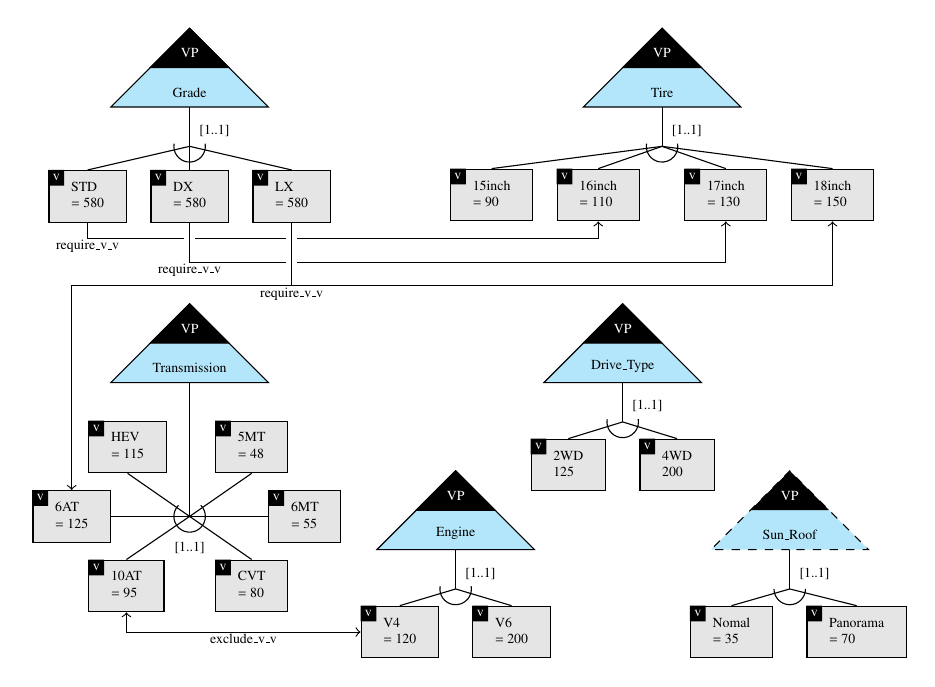
\begin{tikzpicture}
 % Grade
  \nodeVP{grade}{at={(0,0)}}{Grade};
  \nodeV{dx}{below=0.3cm of via_grade}{DX}{= 580};
  \draw(via_grade)--(dx.north);
  \nodeV{std}{left=0.3cm of dx}{STD}{= 580};
  \draw(via_grade)--(std.north);
  \nodeV{lx}{right=0.3cm of dx}{LX}{= 580};
  \draw(via_grade)--(lx.north);

  % Tire
  \nodeVP{tire}{right=6cm of grade}{Tire};
  \nodeV{16inch}{below left=0.4cm of via_tire}{16inch}{= 110};
  \nodeV{17inch}{below right=0.4cm of via_tire}{17inch}{= 130};
  \nodeV{15inch}{left=0.3cm of 16inch}{15inch}{= 90};
  \nodeV{18inch}{right=0.3cm of 17inch}{18inch}{= 150};
  \draw (via_tire)--(15inch.north);
  \draw (via_tire)--(16inch.north);
  \draw (via_tire)--(17inch.north);
  \draw (via_tire)--(18inch.north);

  % Transmission
  \nodeTrans{trans}{below=3.5cm of grade}{Transmission};
  \nodeV{6at}{left=1cm of via_trans}{6AT}{= 125};
  \nodeV{hev}{above right=0.3cm of 6at.north}{HEV}{= 115};
  \nodeV{10at}{below right=0.3cm of 6at.south}{10AT}{= 95};
  \nodeV{6mt}{right=1cm of via_trans}{6MT}{= 55};
  \nodeV{5mt}{above left=0.3cm of 6mt.north}{5MT}{= 48};
  \nodeV{cvt}{below left=0.3cm of 6mt.south}{CVT}{= 80};
  \draw (via_trans)--(10at.north);
  \draw (via_trans)--(6at.east);
  \draw (via_trans)--(hev.south);
  \draw (via_trans)--(6mt.west);
  \draw (via_trans)--(5mt.south);
  \draw (via_trans)--(cvt.north);

  % Drive_Type
  \nodeVP{drivetype}{right=5.5cm of trans}{Drive\_Type};
  \nodeV{2wd}{below left=0.3cm of via_drivetype}{2WD}{125};
  \draw (via_drivetype)--(2wd.north);
  \nodeV{4wd}{below right=0.3cm of via_drivetype}{4WD}{200};
  \draw (via_drivetype)--(4wd.north);


  % Sun_Roof
  \nodeVPdashed{sunroof}{below right=3cm of drivetype}{Sun\_Roof};
  \nodeV{nomal}{below left=0.3cm of via_sunroof}{Nomal}{= 35};
  \draw (via_sunroof)--(nomal.north);
  \nodeV{panorama}{below right=0.3cm of via_sunroof}{Panorama}{= 70};
  \draw (via_sunroof)--(panorama.north);

  % Engine
  \nodeVP{engine}{below left=3cm of drivetype}{Engine};
  \nodeV{v4}{below left=0.3cm of via_engine}{V4}{= 120};
  \draw (via_engine)--(v4.north);
  \nodeV{v6}{below right=0.3cm of via_engine}{V6}{= 200};
  \draw (via_engine)--(v6.north);
  
 

  % require
  \draw[->] (std.south)--++(0,-0.2) node[below=-1mm] {\tiny{require\_v\_v}} -|(16inch.south);
  \draw[white,line width=4pt](dx.south) ++(0,-0.1)--++(0,-0.5);
  \draw[->] (dx.south)--++(0,-0.5) node[below=-1mm] {\tiny{require\_v\_v}} -|(17inch.south);
  \draw[white,line width=4pt] (lx.south) ++(0,-0.1)--++(0,-0.8);
  \draw[->] (lx.south)--++(0,-0.8) node[below=-1mm] {\tiny{require\_v\_v}} -|(18inch.south);
  \draw[->] (lx.south)--++(0,-0.8) -|(6at.north);

  % exclude
  \draw[<->] (v4.west)-|(10at.south) node[pos=0.25,below=-1mm]{\tiny{exclude\_v\_v}};
 \end{tikzpicture}
}
      \uncover<2>{
      \begin{exampleblock}{}\centering
        STD,DX,LXグレードの3車種を生産するとする.
      \end{exampleblock}}
    \end{column}
    \begin{column}{0.25\linewidth}
      \begin{footnotesize}
        \begin{itemize}
        \item プロダクトライン開発で用いられる可変性モデルによって記述
        \item 6個の装備タイプ,19個の装備オプション
        \item 各タイプの選択可能なオプション数はすべて1
        \item 各オプションの数字は IWR 値と呼ばれ,直観的にはその重量
        \item 5個の依存制約
        \item \textsf{Sun Roof}以外は必須タイプ
        \end{itemize}
      \end{footnotesize}
    \end{column}
  \end{columns}
\end{frame}
%%%%%%%%%%%%%%%%%%%%%%%%%%%%%%%%%%%%%%%%%%%%%%%%%%%%
\begin{frame}{CAFE問題の解 {\normalsize (CAFE基準値: 8.5km/L)}}\small
 \begin{exampleblock}{解の例}
  \centering
  \renewcommand{\arraystretch}{0.9}
  %\tabcolsep = 5mm
  \begin{tabular}{p{10mm}|p{25mm}|p{15mm}|p{15mm}|p{15mm}} 
    \multicolumn{2}{l|}{装備仕様}  & 車種1 & 車種2 & 車種3 \\\hline
    装備 & \textsf{Grade}   & \textsf{STD}    & \textsf{DX}     & \textsf{LX}\\
    &\textsf{Drive\_Type}  & \textsf{2WD}    & \textsf{2WD}    & \textsf{4WD}\\
    &\textsf{Engine}	  & \textsf{V6}     & \textsf{V6}     & \textsf{V6}\\
    &\textsf{Tire}	  & \textsf{16inch} & \textsf{17inch} & \textsf{18inch}\\
    &\textsf{Transmission} & \textsf{6AT}    & \textsf{HEV}    & \textsf{10AT}\\
    &\textsf{Sun\_Roof}    & -               & -              & - 
   \end{tabular}
 \end{exampleblock}
 \pause
 
 \begin{block}{}
  \centering
  \renewcommand{\arraystretch}{0.9}
  %\tabcolsep = 5mm
  \begin{tabular}{p{38mm}|p{15mm}|p{15mm}|p{15mm}} 
    IWR 値の総和    & 1,130  & 1,130   & 1,255 \\ %\hline
    燃費(km/L)      & 8.8  & 8.8     & 8.0 \\ %\hline
    予想販売台数    & 2,007   & 2,007   & 1,511  \\ \hline
    平均燃費(km/L)  & \multicolumn{3}{c}{8.5} \\ 
    予想販売台数(合計)  & \multicolumn{3}{c}{5,525} \\ 
    オプション数 & \multicolumn{3}{c}{12}	
  \end{tabular}
 \end{block}
 \vfill
 \begin{itemize}
 \item 車種3はCAFE基準値を下回っているが,
       平均燃費は 8.581km/L となり,燃費制約を満たしている.
 \end{itemize}
\end{frame}
%%%%%%%%%%%%%%%%%%%%%%%%%%%%%%%%%%%%%%%%%%%%%%%%%%%%
\begin{frame}{解集合プログラミング(Anwer Set Programming; ASP)}
 \begin{itemize}
 \item \structure{\bf ASPの言語}は,一階論理に基づく知識表現言語の一種である.
 %\item \structure{\bf ASPのプログラム}は,ASPルールの有限集合である.
 \item \structure{\bf ASPシステム}は,安定モデル意味論~[Gelfond and Lifschitz '88]
   に基づく解集合を計算するシステムである.
 \item 近年,SAT技術を利用した高速なASPシステムが開発され,
   ロボット工学,システム検証,システム生物学
   など様々な分野への実用的応用が急速に拡大している.
  % \item \structure{\bf Asprin言語}は,複数の目的関数およびそれらの間の
  % 	選好(preference)を記述できるようにASP言語を拡張したものである.
 \end{itemize}
\vfill
 \begin{alertblock}{CAFE問題に対してASPを用いる利点}
   \begin{itemize} 
    \item ASP言語の高い表現力により,各種制約を簡潔に記述できる.
    \item 高速なASPシステムを利用できる.
    \item 多目的最適化や,解集合の間の選好順序を記述できるように拡張された
	  \alert{\bf Asprinシステム}[Brewka 15]を利用できる.
    % \item 解の最適性を保証でき,最適解の列挙も可能である.
    % \item Asprin言語の選好により,トレードオフの関係にある複数の目的関数のもとで,
    % 	  柔軟な最適値探索が可能である.
   \end{itemize}
 \end{alertblock}
\end{frame}
%%%%%%%%%%%%%%%%%%%%%%%%%%%%%%%%%%%%%%%%%%%%%%%%%%%%
\begin{frame}{研究の概要}
 \begin{alertblock}{目的}
  \begin{itemize}
   \item   ASPを多目的最適化問題へ応用する試みとして,
	   ASPを基盤とした高速CAFE問題ソルバーを実現する.
   \item 企業から提供を受けたベンチマーク問題を使ってソルバーを評価し,
	 ASPの特長を活かした多目的最適化の利点・実用性を明らかにする.
   % \item CAFE問題のASP符号化の研究開発を中心に研究を進める.
  \end{itemize}
 \end{alertblock}
 \begin{block}{これまでの研究内容}
  \begin{enumerate}
   \item \structure{\bf 単目的CAFE問題に関する研究(卒業研究)}
	 \begin{itemize}
	  \item {\bf 基本符号化}と{\bf 改良符号化}の2種類のASP符号化を考案
	  \item 実用規模,より大規模な問題での{\bf 改良符号化の優位性}を確認
	 \end{itemize}
   \item \structure{\bf 多目的CAFE問題に関する研究}
	 \begin{itemize}
	  \item パレート最適解を求める{\bf 拡張符号化}を考案
	  \item 小規模な問題で,{\bf パレート最適解を全列挙}することに成功
	 \end{itemize}
  \end{enumerate}
 
 \end{block}
\end{frame}
%%%%%%%%%%%%%%%%%%%%%%%%%%%%%%%%%%%%%%%%%%%%%%%%%%%%
\begin{frame}{単目的CAFE問題に関する研究(卒業研究)}
 \begin{block}{}\centering
  目的関数は,予想販売台数の最大化
 \end{block}
 % \begin{block}{}
  \begin{itemize}
   \item {\bf 基本符号化}
	 \begin{itemize}
	  \item CAFE問題の制約を{\bf ASPのルール17個}で簡潔に記述できることを確認した.
	 \end{itemize}
   \item {\bf 改良符号化}
	 \begin{itemize}
	  \item IWR値の上下限を厳密に計算し,
		{\bf 基礎化後のルール数を少なく}抑えるよう工夫されており,
		大規模な問題での有効性が期待できる.
	 \end{itemize}
  \end{itemize}
  % \end{block}
 \begin{exampleblock}{企業から提供された実データを用いた評価実験}
  \begin{itemize}
   \item CAFE問題(3問)に対して,5種類のCAFE基準値(8.5, 9.0, 9.5,
	 10.0, 10.5km/L)を適用した問題インスタンス(全15問)  
   \item どちらの符号化でも小規模な問題の最適解を求めることができた.
   \item 実用規模およびより大規模な問題に対して,
	 改良符号化が基本符号化より優れた結果を示し,その優位性が確認できた.
  \end{itemize}
 \end{exampleblock}

\end{frame}
%%%%%%%%%%%%%%%%%%%%%%%%%%%%%%%%%%%%%%%%%%%%%%%%%%%%
\begin{frame}{多目的CAFE問題に関する研究}
 \begin{block}{}\centering
  目的関数は,予想販売台数の最大化と装備オプション数の最小化
 \end{block}
 \begin{itemize}
  \item {\bf 拡張符号化}
	\begin{itemize}
	 \item 改良符号化をベースに,多目的CAFE問題のパレート最適解を計算できるように拡張
	       されている.
	 \item 2つの目的関数からなる多目的最適化をASPのルール5個で簡潔に記述できることを
	       確認した.
	\end{itemize}
 \end{itemize}
 \begin{exampleblock}{パレート最適解の例{\normalsize (CAFE基準値: 8.5km/L)}}
    \centering
  \tiny
  \tabcolsep=1.5mm
  \begin{tabular}{l|l|c|c|c||c|c|c||c|c|c||c|c|c}
   \multicolumn{2}{l|}{} & \multicolumn{3}{c||}{解1} & \multicolumn{3}{c||}{解2} & \multicolumn{3}{c||}{解3} & \multicolumn{3}{c}{解4}\\ \hline
   \multicolumn{2}{l|}{装備仕様} & 1 & 2 & 3 & 1 & 2 & 3 & 1 & 2 & 3 & 1 & 2 & 3 \\ \hline
   装備 & Grade & STD & DX & LX & STD & DX & LX & STD & DX & LX & STD & DX & LX \\
       & Drive\_Type & 2WD & 2WD & \alert{4WD} & 2WD & 2WD & \alert{4WD} & 2WD & 2WD & \alert{2WD} & 2WD & 2WD & \alert{2WD}\\
       & Engine & V6 & V6 & V6 & V6 & V6 & V6 & V6 & V6 & V6 & V6 & V6 & V6 \\
       & Tire & 16 & 17 & 18 & 16 & 17 & 18 & 16 & 17 & 18 & 16 & 17 & 18 \\
       & Transmission & \alert{6AT} & \alert{HEV} & 10AT & \alert{10AT} & \alert{HEV} & 10AT & \alert{10AT} & \alert{HEV} & 10AT & \alert{10AT} & \alert{10AT} & 10AT \\
       & Sun\_Roof & - & - & - & - & - & - & - & - & - & - & - & - \\ \hline
   \multicolumn{2}{l|}{予想販売台数(合計)}  & \multicolumn{3}{c||}{\bf 5,525} & \multicolumn{3}{c||}{\bf 5,475} & \multicolumn{3}{c||}{\bf 5,135} & \multicolumn{3}{c}{\bf 4,723} \\ 
   \multicolumn{2}{l|}{オプション数} & \multicolumn{3}{c||}{\bf 12} & \multicolumn{3}{c||}{\bf 11} & \multicolumn{3}{c||}{\bf 10} & \multicolumn{3}{c}{\bf 9} \\
   \multicolumn{14}{c}{}
  \end{tabular}

 \end{exampleblock}
\end{frame}
%%%%%%%%%%%%%%%%%%%%%%%%%%%%%%%%%%%%%%%%%%%%%%%%%%%%
\begin{frame}{実験概要}
 \begin{itemize}
  \item 考案した拡張符号化の有効性を評価するために,実行実験を行った.
% 問題の規模がわかるように	
 \end{itemize}

\begin{itemize}
\item ベンチマーク問題(計15問)
  \begin{itemize}
  \item 企業から提供された問題(3問)に対して
  \item 5通りのCAFE基準値$t\in\{8.5, 9.0, 9.5, 10.0, 10.5km/L\}$を適用
  \item 車種の数$n = 3$
  \end{itemize}
  \begin{exampleblock}\small
    \centering
    \begin{tabular}{ ll|r r r }
      問題名 & サイズ &  \#装備タイプ & \#装備オプション& \#依存制約\\ \hline
      small	 & 小規模   &   8 &   21  &   4	\\
      medium & 実用規模 &  86 &  226  & 147	\\
      big    & 大規模   & 315 & 1,337 &   0
    \end{tabular}
  \end{exampleblock}
 \item ASPシステム
       \begin{itemize}
	\item \textit{clingo-5.4.0} + \textit{asprin-3.1.1}
       \end{itemize}
 \item 制限時間
       \begin{itemize}
	\item 1問あたり3時間
       \end{itemize}
 \item 実験環境: Mac mini (3.2GHz, Intel Core i7, 64GB メモリ)
\end{itemize}
\end{frame}
%%%%%%%%%%%%%%%%%%%%%%%%%%%%%%%%%%%%%%%%%%%%%%%%%%%%
\begin{frame}{小規模な問題での実験結果}
 \begin{exampleblock}{}
  \centering
  % \renewcommand{\arraystretch}{0.9}
  % \tabcolsep = 0.9mm
  \begin{tabular}{c|r|rr}
   問題   & CAFE値  & パレート最適解 & CPU時間(秒) \\
          & (km/L)  & の総数  &  \\ \hline
   small  & 8.5   & 8             & 35.136     \\
   small  & 9.0   & 5             & 1085.354   \\
   small  & 9.5   & --            & Timeout    \\
   small  & 10.0  & 1             & 1.863      \\
   small  & 10.5  & 0             & 0.221      \\ 
  \end{tabular}
 \end{exampleblock}
 \begin{itemize}
  \item 5問中4問でパレート最適解を全列挙することに成功した.
  \item medium 以上の問題では暫定的な解は得られたが,最適解は得られなかった.
 \end{itemize}
\end{frame}
%%%%%%%%%%%%%%%%%%%%%%%%%%%%%%%%%%%%%%%%%%%%%%%%%%%%
\begin{frame}{まとめと今後の課題}
 解集合プログラミングを用いたCAFE問題の解法について,
 研究概要とこれまでの研究成果を述べた.
 \begin{block}{これまでの研究内容}
  \begin{itemize}
   \item \structure{\bf 単目的CAFE問題に関する研究(卒業研究)}
	 \begin{itemize}
	  \item {\bf 基本符号化}と{\bf 改良符号化}の2種類のASP符号化を考案した.
	  \item 実用規模,より大規模な問題での改良符号化の優位性を確認した.
	 \end{itemize}
   \item \structure{\bf 多目的CAFE問題に関する研究}
	 \begin{itemize}
	  \item パレート最適解を求める{\bf 拡張符号化}を考案した.
	  \item 小規模な問題でのパレート最適解を全列挙することに成功した.
	 \end{itemize}
  \end{itemize}
 \end{block}
 \begin{alertblock}{今後の課題}
  認証制約,
  適用タイミング制約,
  IWRテーブル制約
  など,CAFE 問題に対する様々な追加制約に対応し,
  ソルバーの実用性を高める.

 \end{alertblock}
\end{frame}
%%%%%%%%%%%%%%%%%%%%%%%%%%%%%%%%%%%%%%%%%%%%%%%%%%%%
\begin{frame}{研究業績}
 \begin{alertblock}{受賞}
  \begin{itemize}
   \item {\bf 学生奨励賞}\\
	 竹内頼人, 田村直之, 番原睦則.
	 車両装備仕様問題に対する解集合プログラミングの適用.
	 日本ソフトウェア科学会第37回大会講演論文集,
	 2020年9月9日. 
  \end{itemize}
 \end{alertblock}
 \begin{block}{今後の発表予定}
  \begin{itemize}
   \item 竹内頼人, 田村直之, 番原睦則. 解集合プログラミングを用いた多目的車両装備仕様問題の解法. 2021年度人工知能学会全国大会(第35回), 2020年6月. 
  \end{itemize}
 \end{block}
 \begin{exampleblock}{研究会等での口頭発表}
   \begin{itemize}
    \item 2020/9/3 NII共同研究 第1回研究会合
    % \item 2020/9/9 日本ソフトウェア科学会 第37回大会
    \item 2020/10/16 企業とのCAFE問題に関する意見交換会
   \end{itemize} 
 \end{exampleblock}
\end{frame}
%%%%%%%%%%%%%%%%%%%%%%%%%%%%%%%%%%%%%%%%%%%%%%%%%%%%
\appendix
\backupbegin
%%%%%%%%%%%%%%%%%%%%%%%%%%%%%%%%%%%%%%%%%%%%%%%%%%%%
\begin{frame}{単目的CAFE問題の実験結果:予想販売台数}
\begin{exampleblock}{}
  \centering
  \scriptsize
  \renewcommand{\arraystretch}{1.1}
  \tabcolsep = 7mm
  \begin{tabular}{l|r|rr}
  \lw{問題名} & CAFE  & \multicolumn{2}{c}{予想販売台数} \\ \cline{3-4}
              & 基準値 & 基本符号化 & 改良符号化 \\\hline    
   small & 8.5   & \alert{6,021*} & \alert{6,021*}       \\
   small & 9.0   & \alert{5,007*} & \alert{5,007*}       \\
   small & 9.5   & \alert{2,688*} & \alert{2,688*}       \\
   small & 10.0  & \alert{1,318*} & \alert{1,318*}       \\
   small & 10.5  & UNSAT          & UNSAT    \\\hline
   medium & 8.5  & 6,010          & \alert{6,021}        \\
   medium & 9.0  & \alert{5,595}  & \alert{5,595}        \\
   medium & 9.5  & \alert{3,447}  & 3,430        \\
   medium & 10.0 & 2,245          & \alert{2,250}        \\
   medium & 10.5 & 1,690          & \alert{1,845}        \\\hline
   big & 8.5     & -             & \alert{3,877}        \\
   big & 9.0     & 1,038          & \alert{4,623}        \\
   big & 9.5     & 688            & \alert{3,121}        \\
   big & 10.0    & 1,634          & \alert{2,064}        \\
   big & 10.5    & 538            & \alert{904}         \\\hline
   \multicolumn{2}{l}{最適値・最良値の数} & \multicolumn{1}{r}{6} & \alert{13} \\
  \end{tabular}
\end{exampleblock}
\vfill
\begin{itemize}%\small
\item 改良符号化が,より多くの問題に対して優れた結果を示した.
\item 特に,大規模な問題に対する改良符号化の優位性が確認できた.
 \end{itemize}	
\end{frame}
%%%%%%%%%%%%%%%%%%%%%%%%%%%%%%%%%%%%%%%%%%%%%%%%%%%%
\begin{frame}{単目的CAFE問題の実験結果: 求解までのCPU時間}
  
\begin{exampleblock}{}\centering 
  \renewcommand{\arraystretch}{1.2}
  \tabcolsep = 4mm
  \begin{tabular}{cc|r|rr}
    \lw{問題名} & \lw{結果} & CAFE  & \multicolumn{2}{c}{CPU時間(秒)} \\ \cline{4-5}
             &  & 基準値 & 基本符号化 & 改良符号化 \\\hline
    small  & OPT &  8.5  & 37.868         & \alert{23.318}  \\
    small  & OPT &  9.0  & 48.965         & \alert{43.362}  \\
    small  & OPT &  9.5  & \alert{95.110} & 173.172         \\
    small  & OPT & 10.0  & 99.954         & \alert{0.343}   \\
    small  & UNSAT   & 10.5  & 439.613        & \alert{0.080}   \\\hline
   \multicolumn{3}{r}{平均}  & 144.302        & \alert{48.055}
  \end{tabular}
\end{exampleblock}
\begin{itemize}
\item 5問中4問に対して,改良符号化がより高速に解を求めている.
%\item 平均では,改良符号化のCPU時間は基本符号化の約1/3であった.
\end{itemize}
\end{frame}
%%%%%%%%%%%%%%%%%%%%%%%%%%%%%%%%%%%%%%%%%%%%%%%%%%%%
\begin{frame}{CAFE問題ソルバーの構成}
 \scalebox{0.9}{\centering  \thicklines
  \setlength{\unitlength}{1.28pt}
  \small
  \begin{picture}(280,57)(4,-10)
    \put(  0, 20){\dashbox(50,24){\shortstack{根付き全域森\\問題}}}
    \put( 60, 20){\framebox(50,24){変換器}}
    \put(120, 20){\dashbox(50,24){\shortstack{ASPファクト}}}
    \put(120,-10){\alert{\bf\dashbox(50,24){\scriptsize{\shortstack{ASP符号化\\(論理プログラム)}}}}}
    \put(180, 20){\framebox(50,24){ASPシステム}}
    \put(240, 20){\dashbox(50,24){\shortstack{根付き全域森\\問題の解}}}
    \put( 50, 32){\vector(1,0){10}}
    \put(110, 32){\vector(1,0){10}}
    \put(170, 32){\vector(1,0){10}}
    \put(230, 32){\vector(1,0){10}}
    \put(170, +2){\line(1,0){4}}
    \put(174, +2){\line(0,1){30}}
  \end{picture}  
}
\end{frame}
%%%%%%%%%%%%%%%%%%%%%%%%%%%%%%%%%%%%%%%%%%%%%%%%%%%%
\backupend
\end{document}